
\subsection{Verwendung einer GUI}

Der Aufruf mittels Befehleingabe im Terminal zeigte sich als dauerhaft zu umständlich. Ständiges Wechseln der Pfade, gestaltete sich ebenso störend, wie die Eingabe der Befehle, die mal mit, mal ohne Root-Rechte gestartet werden konnten. Aus diesen Grund erstellten wir Shellskripte, die ein unnötiges hantieren im Terminal verhindern sollte. Aber auch diese Lösung gefiel uns nicht. Da wir teilweise an verschiedenen Rechnern verschiedene Konzepte umgesetzt hatten, aber jede Gruppe ihren Testbedarf hatte, musste unser GSM-Netz oftmals eingeschaltet und kurz darauf wieder abgeschalten werden. Jeder Einschaltvorgang bestand dabei mindestens aus vier Terminalfenster in denen die Startskripte aufgerufen werden mussten. Zudem musste dies in richtiger Reihenfolge geschehen. Abhilfe schaffte hier eine einfache GUI-Anwendung, die mit Hilfe von Qt in C++ verfasst wurde.  

\begin{figure}[h] %t=top b=bottom h=here p =eigene page
\centering
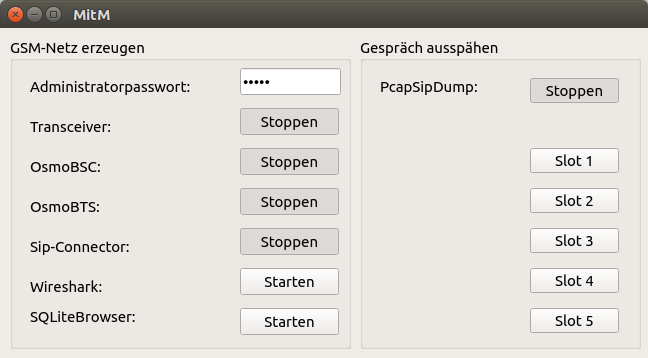
\includegraphics[width=15cm]{includes/gui}
\caption{GUI-Anwendung MitM}
\label{fig:GUI}
\end{figure}


Diese besteht im wesentlichen aus zwei Seiten. Die linke Seite beinhaltet zahlreiche Toggle-Buttons, mit denen die vorhandenen Shellskripte aufgerufen werden. Sie schalten die jeweilige Anwendung ein oder aus. Zudem ist ein Eingabefeld für das Root-Passwort vorhanden, da etliche Anwendungen Root-Rechte benötigen. Allerdings konnte dies nicht mehr fertiggestellt werden, so dass die Eingabe des Passworts derzeit wirkungslos bleibt. Stattdessen muss die GUI-Anwendung selbst mit Root-Rechten gestartet werden. Die linke Seite dient daher der Erzeugung eines GSM-Netzes. 
Auf der rechten Seite hingegen, befinden sich die Buttons mit denen ein Gespräch ausgespäht werden kann. Mit den Toggle-Button "PcapSipDump" wird das Shellskript gestartet, welches die Gespräche abfängt und in Audiostreams umwandelt. Die zugehörigen Buttons "Slot 1 -5" geben diese Gespräche wieder. 
Nachfolgend ist der Quellcode der GUI-Anwendung aufgelistet:
\vspace{1cm}

\textbf{Inhalt von main.cpp}

\begin{lstlisting}
#include "mitm.h"
#include <QApplication>

int main(int argc, char *argv[])
{
    QApplication a(argc, argv);
    MitM w;
    w.show();

    return a.exec();
}
\end{lstlisting}



\vspace{2cm}
\textbf{Inhalt von mitm.h}



\begin{lstlisting}
#ifndef MITM_H
#define MITM_H

#include <QMainWindow>
#include <QProcess>

namespace Ui {
class MitM;
}

class MitM : public QMainWindow
{
    Q_OBJECT

public:
    explicit MitM(QWidget *parent = 0);
    ~MitM();

private:
    Ui::MitM *ui;
    QString password;

public slots:
    void checkInput();
    void transceiverPressed();
    void btsPressed();
    void bscPressed();
    void wiresharkPressed();
    void sipConnectorPressed();
    void sqlBrowserPressed();
    void pcapSipDumpPressed();
    void slot1Pressed();
    void slot2Pressed();
    void slot3Pressed();
    void slot4Pressed();
    void slot5Pressed();
};
#endif // MITM_H
\end{lstlisting}



\vspace{2cm}
\textbf{Inhalt von mitm.cpp}

\begin{lstlisting}
#include "mitm.h"
#include "ui_mitm.h"

MitM::MitM(QWidget *parent) :
    QMainWindow(parent),
    ui(new Ui::MitM)
{
    ui->setupUi(this);

    connect(ui->lineEdit, SIGNAL(textEdited(QString)), this, SLOT(checkInput()));
    connect(ui->pushButtonTransceiver, SIGNAL(clicked()), this, SLOT(transceiverPressed()));
    connect(ui->pushButtonBSC, SIGNAL(clicked()), this, SLOT(bscPressed()));
    connect(ui->pushButtonBTS, SIGNAL(clicked()), this, SLOT(btsPressed()));
    connect(ui->pushButtonSipConnector, SIGNAL(clicked()), this, SLOT(sipConnectorPressed()));
    connect(ui->pushButtonWireshark, SIGNAL(clicked()), this, SLOT(wiresharkPressed()));
    connect(ui->pushButtonSQLBrowser, SIGNAL(clicked()), this, SLOT(sqlBrowserPressed()));
    connect(ui->pushButtonPcap, SIGNAL(clicked()), this, SLOT(pcapSipDumpPressed()));
    connect(ui->pushButtonSlot1, SIGNAL(clicked()), this, SLOT(slot1Pressed()));
    connect(ui->pushButtonSlot2, SIGNAL(clicked()), this, SLOT(slot2Pressed()));
    connect(ui->pushButtonSlot3, SIGNAL(clicked()), this, SLOT(slot3Pressed()));
    connect(ui->pushButtonSlot4, SIGNAL(clicked()), this, SLOT(slot4Pressed()));
    connect(ui->pushButtonSlot5, SIGNAL(clicked()), this, SLOT(slot5Pressed()));
}


MitM::~MitM()
{
    delete ui;
}


void MitM::checkInput() {
    password = ui->lineEdit->text();
}


void MitM::transceiverPressed(){

    QProcess* exec = new QProcess(this);

    if (ui->pushButtonTransceiver->isChecked()) {
        exec->start("./startTransceiver.sh");
        ui->pushButtonTransceiver->setText("Stoppen");
    }
    else {
        exec->close();
        ui->pushButtonTransceiver->setText("Starten");
    }
}



void MitM::bscPressed(){

    QProcess* exec = new QProcess(this);

    if (ui->pushButtonBSC->isChecked()) {
        exec->start("./startOsmoNitb.sh");
        ui->pushButtonBSC->setText("Stoppen");
    }
    else {
        exec->close();
        ui->pushButtonBSC->setText("Starten");
    }
}


void MitM::btsPressed(){

    QProcess* exec = new QProcess(this);

    if (ui->pushButtonBTS->isChecked()) {
        exec->start("./startOsmoBTS.sh");
        ui->pushButtonBTS->setText("Stoppen");
    }
    else {
        exec->close();
        ui->pushButtonBTS->setText("Starten");
    }
}



void MitM::wiresharkPressed(){

    QProcess* exec = new QProcess(this);

    if (ui->pushButtonWireshark->isChecked()) {
        exec->start("./wireshark.sh");
        ui->pushButtonWireshark->setText("Stoppen");
    }
    else {
        exec->close();
        ui->pushButtonWireshark->setText("Starten");
    }
}



void MitM::sipConnectorPressed(){

    QProcess* exec = new QProcess(this);

    if (ui->pushButtonSipConnector->isChecked()) {
        exec->start("./startSipConnector.sh");
        ui->pushButtonSipConnector->setText("Stoppen");
    }
    else {
        exec->close();
        ui->pushButtonSipConnector->setText("Starten");
    }
}



void MitM::sqlBrowserPressed(){

    QProcess* exec = new QProcess(this);

    if (ui->pushButtonSQLBrowser->isChecked()) {
        exec->start("./startSQLBrowser.sh");
        ui->pushButtonSQLBrowser->setText("Stoppen");
    }
    else {
        exec->close();
        ui->pushButtonSQLBrowser->setText("Starten");
    }
}



void MitM::pcapSipDumpPressed(){

    QProcess* exec = new QProcess(this);

    if (ui->pushButtonPcap->isChecked()) {
        exec->start("./startPcapSipDump.sh");
        ui->pushButtonPcap->setText("Stoppen");
    }
    else {
        exec->close();
        ui->pushButtonPcap->setText("Starten");
    }
}


void MitM::slot1Pressed(){
    QProcess* exec = new QProcess(this);
    exec->start("./slot1.sh");
}

void MitM::slot2Pressed(){
    QProcess* exec = new QProcess(this);
    exec->start("./slot2.sh");
}

void MitM::slot3Pressed(){
    QProcess* exec = new QProcess(this);
    exec->start("./slot3.sh");
}

void MitM::slot4Pressed(){
    QProcess* exec = new QProcess(this);
    exec->start("./slot4.sh");
}

void MitM::slot5Pressed(){
    QProcess* exec = new QProcess(this);
    exec->start("./slot5.sh");
}
\end{lstlisting}


\vspace{2cm}
\textbf{Inhalt von mitm.ui}

\begin{lstlisting}
<?xml version="1.0" encoding="UTF-8"?>
<ui version="4.0">
 <class>MitM</class>
 <widget class="QMainWindow" name="MitM">
  <property name="geometry">
   <rect>
    <x>0</x>
    <y>0</y>
    <width>648</width>
    <height>330</height>
   </rect>
  </property>
  <property name="windowTitle">
   <string>MitM</string>
  </property>
  <widget class="QWidget" name="centralWidget">
   <widget class="QGroupBox" name="groupBox">
    <property name="geometry">
     <rect>
      <x>10</x>
      <y>10</y>
      <width>341</width>
      <height>311</height>
     </rect>
    </property>
    <property name="title">
     <string>GSM-Netz erzeugen</string>
    </property>
    <widget class="QLabel" name="label">
     <property name="geometry">
      <rect>
       <x>20</x>
       <y>40</y>
       <width>171</width>
       <height>17</height>
      </rect>
     </property>
     <property name="text">
      <string>Administratorpasswort:</string>
     </property>
    </widget>
    <widget class="QPushButton" name="pushButtonWireshark">
     <property name="geometry">
      <rect>
       <x>230</x>
       <y>230</y>
       <width>99</width>
       <height>27</height>
      </rect>
     </property>
     <property name="text">
      <string>Starten</string>
     </property>
     <property name="checkable">
      <bool>true</bool>
     </property>
    </widget>
    <widget class="QLabel" name="label_4">
     <property name="geometry">
      <rect>
       <x>20</x>
       <y>160</y>
       <width>81</width>
       <height>17</height>
      </rect>
     </property>
     <property name="text">
      <string>OsmoBTS:</string>
     </property>
    </widget>
    <widget class="QLabel" name="label_6">
     <property name="geometry">
      <rect>
       <x>20</x>
       <y>240</y>
       <width>91</width>
       <height>17</height>
      </rect>
     </property>
     <property name="text">
      <string>Wireshark:</string>
     </property>
    </widget>
    <widget class="QLabel" name="label_2">
     <property name="geometry">
      <rect>
       <x>20</x>
       <y>80</y>
       <width>111</width>
       <height>17</height>
      </rect>
     </property>
     <property name="text">
      <string>Transceiver:</string>
     </property>
    </widget>
    <widget class="QLabel" name="label_3">
     <property name="geometry">
      <rect>
       <x>20</x>
       <y>120</y>
       <width>91</width>
       <height>17</height>
      </rect>
     </property>
     <property name="text">
      <string>OsmoBSC:</string>
     </property>
    </widget>
    <widget class="QPushButton" name="pushButtonSipConnector">
     <property name="geometry">
      <rect>
       <x>230</x>
       <y>190</y>
       <width>99</width>
       <height>27</height>
      </rect>
     </property>
     <property name="text">
      <string>Starten</string>
     </property>
     <property name="checkable">
      <bool>true</bool>
     </property>
    </widget>
    <widget class="QPushButton" name="pushButtonSQLBrowser">
     <property name="geometry">
      <rect>
       <x>230</x>
       <y>270</y>
       <width>99</width>
       <height>27</height>
      </rect>
     </property>
     <property name="text">
      <string>Starten</string>
     </property>
     <property name="checkable">
      <bool>true</bool>
     </property>
    </widget>
    <widget class="QLineEdit" name="lineEdit">
     <property name="geometry">
      <rect>
       <x>230</x>
       <y>30</y>
       <width>101</width>
       <height>27</height>
      </rect>
     </property>
     <property name="echoMode">
      <enum>QLineEdit::Password</enum>
     </property>
    </widget>
    <widget class="QPushButton" name="pushButtonTransceiver">
     <property name="geometry">
      <rect>
       <x>230</x>
       <y>70</y>
       <width>99</width>
       <height>27</height>
      </rect>
     </property>
     <property name="text">
      <string>Starten</string>
     </property>
     <property name="checkable">
      <bool>true</bool>
     </property>
    </widget>
    <widget class="QLabel" name="label_5">
     <property name="geometry">
      <rect>
       <x>20</x>
       <y>200</y>
       <width>111</width>
       <height>17</height>
      </rect>
     </property>
     <property name="text">
      <string>Sip-Connector:</string>
     </property>
    </widget>
    <widget class="QPushButton" name="pushButtonBTS">
     <property name="geometry">
      <rect>
       <x>230</x>
       <y>150</y>
       <width>99</width>
       <height>27</height>
      </rect>
     </property>
     <property name="text">
      <string>Starten</string>
     </property>
     <property name="checkable">
      <bool>true</bool>
     </property>
    </widget>
    <widget class="QPushButton" name="pushButtonBSC">
     <property name="geometry">
      <rect>
       <x>230</x>
       <y>110</y>
       <width>99</width>
       <height>27</height>
      </rect>
     </property>
     <property name="text">
      <string>Starten</string>
     </property>
     <property name="checkable">
      <bool>true</bool>
     </property>
    </widget>
    <widget class="QLabel" name="label_7">
     <property name="geometry">
      <rect>
       <x>20</x>
       <y>270</y>
       <width>121</width>
       <height>17</height>
      </rect>
     </property>
     <property name="text">
      <string>SQLiteBrowser:</string>
     </property>
    </widget>
   </widget>
   <widget class="QGroupBox" name="groupBox_2">
    <property name="geometry">
     <rect>
      <x>360</x>
      <y>10</y>
      <width>281</width>
      <height>311</height>
     </rect>
    </property>
    <property name="title">
     <string>Gesprach ausspahen</string>
    </property>
    <widget class="QLabel" name="label_8">
     <property name="geometry">
      <rect>
       <x>20</x>
       <y>40</y>
       <width>111</width>
       <height>17</height>
      </rect>
     </property>
     <property name="text">
      <string>PcapSipDump:</string>
     </property>
    </widget>
    <widget class="QPushButton" name="pushButtonPcap">
     <property name="geometry">
      <rect>
       <x>170</x>
       <y>40</y>
       <width>89</width>
       <height>25</height>
      </rect>
     </property>
     <property name="text">
      <string>Starten</string>
     </property>
     <property name="checkable">
      <bool>true</bool>
     </property>
    </widget>
    <widget class="QPushButton" name="pushButtonSlot1">
     <property name="geometry">
      <rect>
       <x>170</x>
       <y>110</y>
       <width>89</width>
       <height>25</height>
      </rect>
     </property>
     <property name="text">
      <string>Slot 1</string>
     </property>
    </widget>
    <widget class="QPushButton" name="pushButtonSlot2">
     <property name="geometry">
      <rect>
       <x>170</x>
       <y>150</y>
       <width>89</width>
       <height>25</height>
      </rect>
     </property>
     <property name="text">
      <string>Slot 2</string>
     </property>
    </widget>
    <widget class="QPushButton" name="pushButtonSlot3">
     <property name="geometry">
      <rect>
       <x>170</x>
       <y>190</y>
       <width>89</width>
       <height>25</height>
      </rect>
     </property>
     <property name="text">
      <string>Slot 3</string>
     </property>
    </widget>
    <widget class="QPushButton" name="pushButtonSlot4">
     <property name="geometry">
      <rect>
       <x>170</x>
       <y>230</y>
       <width>89</width>
       <height>25</height>
      </rect>
     </property>
     <property name="text">
      <string>Slot 4</string>
     </property>
    </widget>
    <widget class="QPushButton" name="pushButtonSlot5">
     <property name="geometry">
      <rect>
       <x>170</x>
       <y>270</y>
       <width>89</width>
       <height>25</height>
      </rect>
     </property>
     <property name="text">
      <string>Slot 5</string>
     </property>
    </widget>
   </widget>
  </widget>
 </widget>
 <layoutdefault spacing="6" margin="11"/>
 <resources/>
 <connections/>
</ui>
\end{lstlisting}
